\section{Time Comparison}
With the same approach explained in Section 3, times have been calculated. Figure \ref{fig:timeNC} and \ref{fig:timeH} provides plots for the execution time counting only the time needed for doing merge operations (not the whole execution of the program!). As expected, Quick-Union without path compression performs the worst when we compare with weighted unions (the difference is even more clear as we increase the size of the data structure). Still, with weighted unions we see that time is getting more close to each other as we increase the size (but this is not a surprise, as time execution is related to average TPL and TPU which has been calculated in the previous section, where we saw that both metrics are similar using weighted unions).

\begin{figure}[ht]
    \centering
    % Subfigure 1
    \begin{subfigure}{0.32\textwidth}
        \centering
        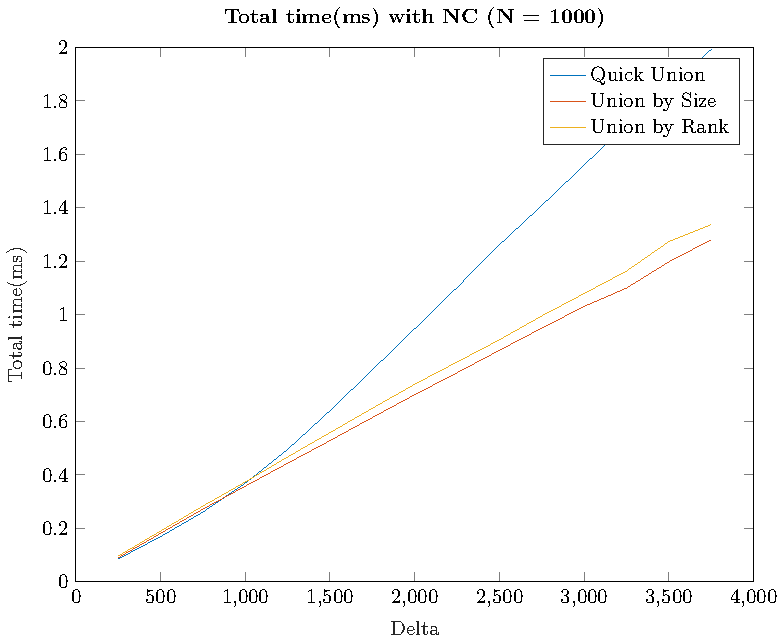
\includegraphics[width=\textwidth]{../images/plotNCFull1000_time(ms).pdf}
        \caption{Total time with different union strategies with $n = 1000$}
    \end{subfigure}%
    \hfill
    % Subfigure 2
    \begin{subfigure}{0.32\textwidth}
        \centering
        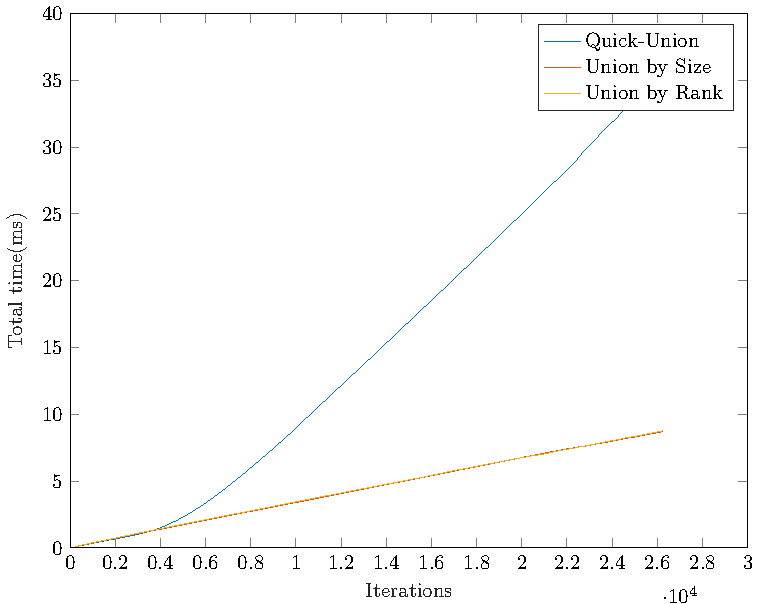
\includegraphics[width=\textwidth]{../images/plotNCFull5000_time(ms).pdf}
        \caption{Total Time with different union strategies with $n = 5000$}
    \end{subfigure}%
    \hfill
    % Subfigure 3
    \begin{subfigure}{0.32\textwidth}
        \centering
        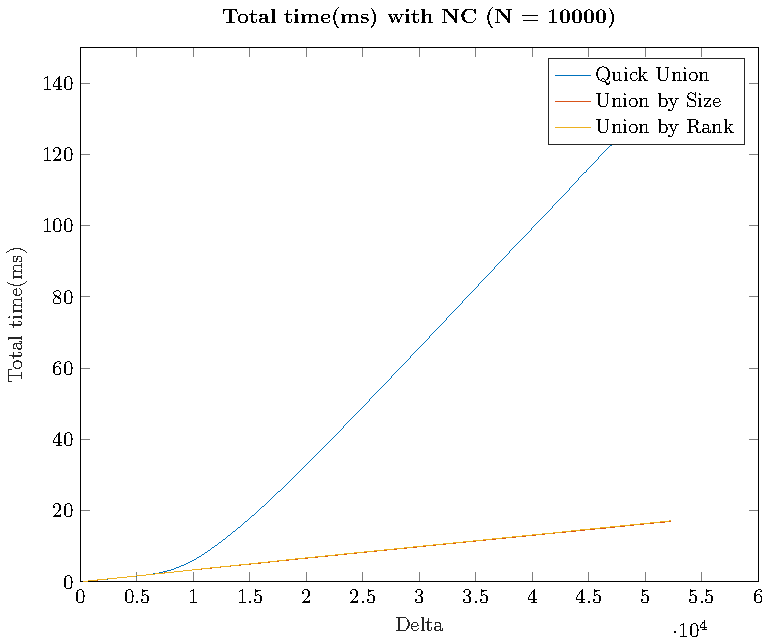
\includegraphics[width=\textwidth]{../images/plotNCFull10000_time(ms).pdf}
        \caption{Total Time with different union strategies with $n = 10000$}
    \end{subfigure}
    \begin{subfigure}{0.32\textwidth}
        \centering
        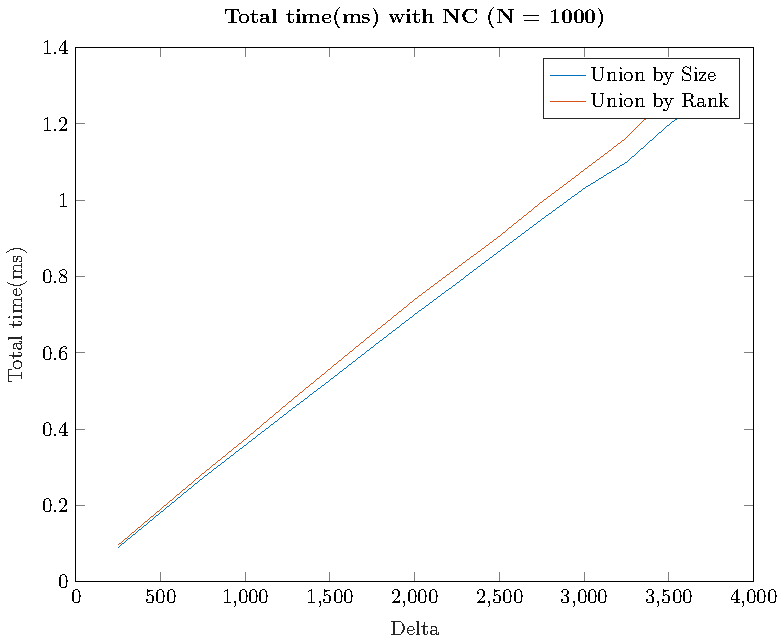
\includegraphics[width=\textwidth]{../images/plotNCNonFull1000_time(ms).pdf}
        \caption{Total Time with different union strategies with $n = 1000$ without Quick-Union}
    \end{subfigure}%
    \hfill
    % Subfigure 2
    \begin{subfigure}{0.32\textwidth}
        \centering
        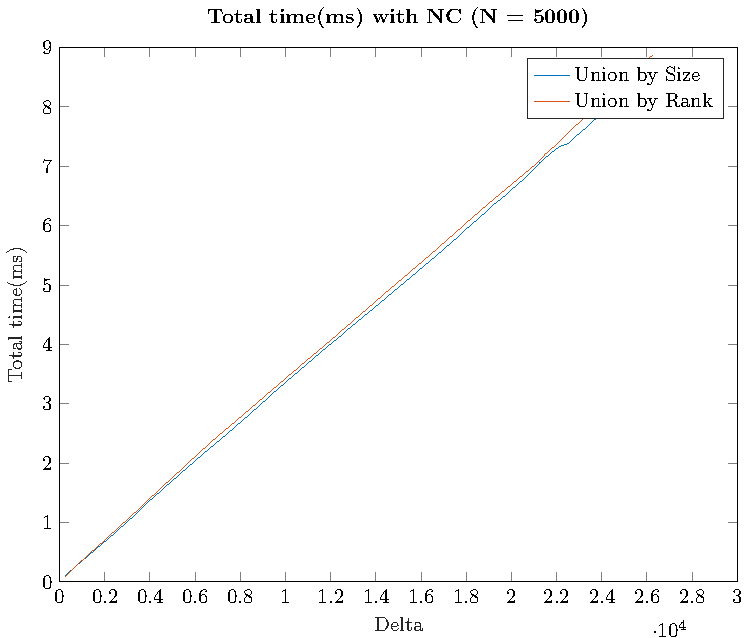
\includegraphics[width=\textwidth]{../images/plotNCNonFull5000_time(ms).pdf}
        \caption{Total Time with different union strategies with $n = 5000$ without Quick-Union}
    \end{subfigure}%
    \hfill
    % Subfigure 3
    \begin{subfigure}{0.32\textwidth}
        \centering
        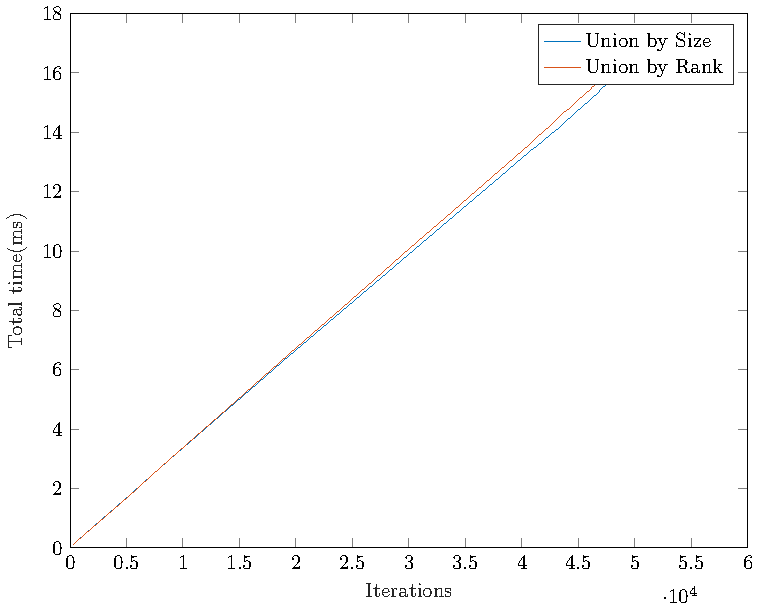
\includegraphics[width=\textwidth]{../images/plotNCNonFull10000_time(ms).pdf}
        \caption{Total Time with different union strategies with $n = 10000$ without Quick-Union}
    \end{subfigure}

    \caption{Total time No Compression}
    \label{fig:timeNC}
\end{figure}


What is really interesting is that when we add path compression techniques, although Quick-Union performed the worst in both TPL and TPU metrics using any path heuristic, its execution time does not notably differ from weighted unions (see Figure \ref{fig:timeH}), as TPL and TPU do. We might need a larger sample size to spot a notable difference in the trade-off of performing \textit{cheap} unions in exchange for letting the find operation balance the trees. In fact there is not a noticable difference in execution time rather than calculating metrics.
\begin{figure}[ht]
    \centering
    \begin{subfigure}{0.32\textwidth}
        \centering
        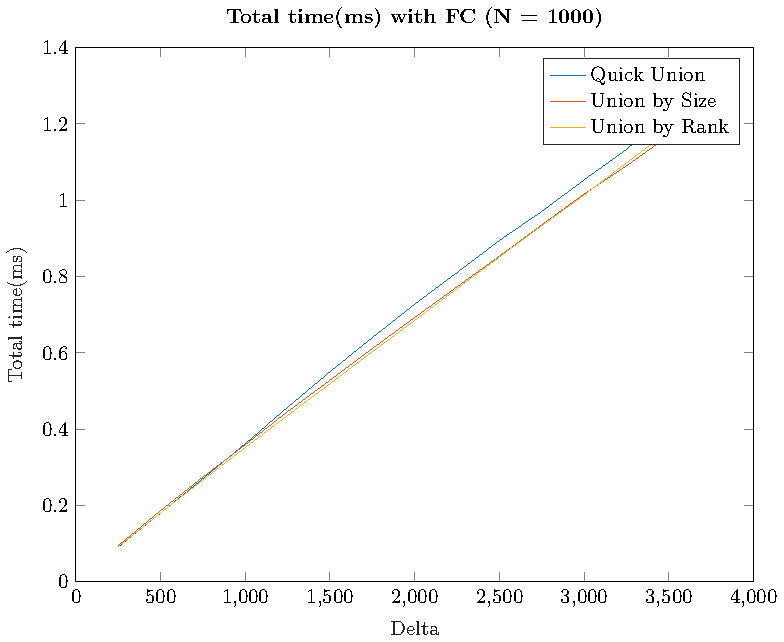
\includegraphics[width=\textwidth]{../images/plotFCFull1000_time(ms).pdf}
        \caption{Total Time with different union strategies with $n = 1000$ using Full Compression}
    \end{subfigure}%
    \hfill
    % Subfigure 2
    \begin{subfigure}{0.32\textwidth}
        \centering
        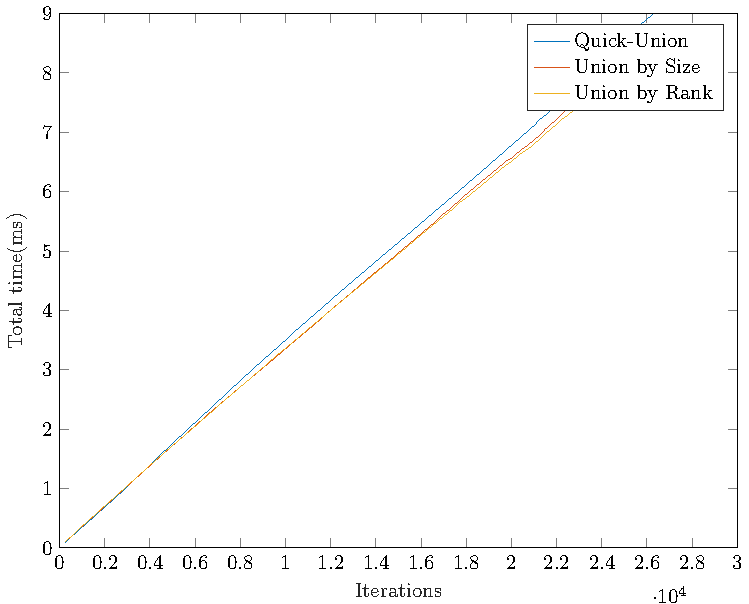
\includegraphics[width=\textwidth]{../images/plotFCFull5000_time(ms).pdf}
        \caption{Total Time with different union strategies with $n = 5000$ using Full Compression}
    \end{subfigure}%
    \hfill
    % Subfigure 3
    \begin{subfigure}{0.32\textwidth}
        \centering
        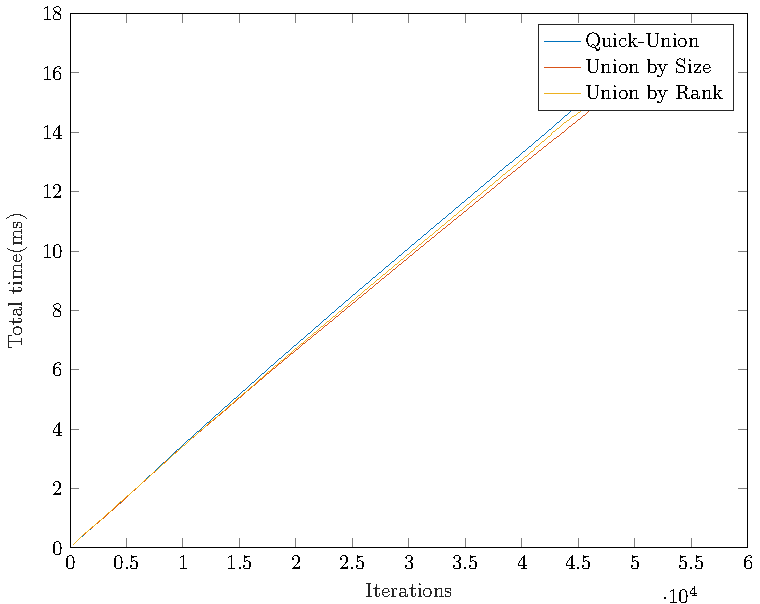
\includegraphics[width=\textwidth]{../images/plotFCFull10000_time(ms).pdf}
        \caption{Total Time with different union strategies with $n = 10000$ using Full Compression}
    \end{subfigure}
    % Subfigure 1
    \begin{subfigure}{0.32\textwidth}
        \centering
        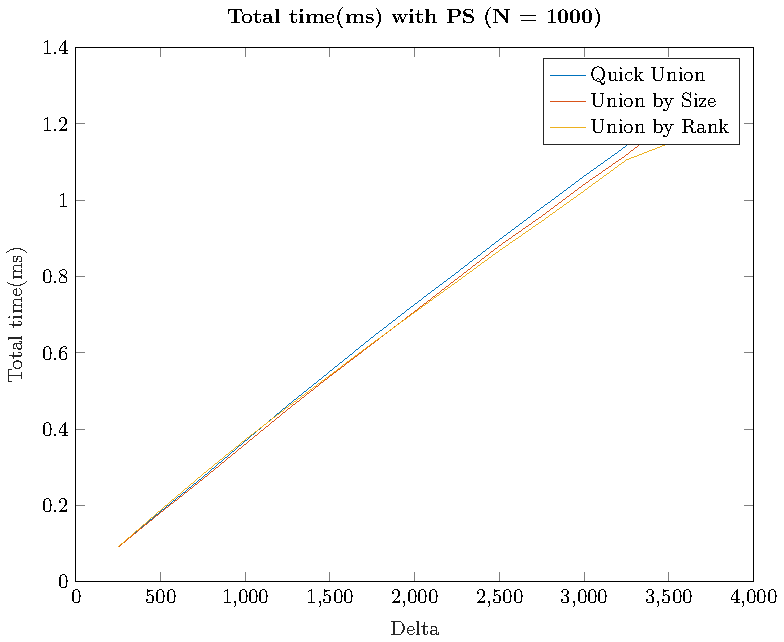
\includegraphics[width=\textwidth]{../images/plotPSFull1000_time(ms).pdf}
        \caption{Total Time with different union strategies with $n = 1000$ using Path Splitting}
    \end{subfigure}%
    \hfill
    % Subfigure 2
    \begin{subfigure}{0.32\textwidth}
        \centering
        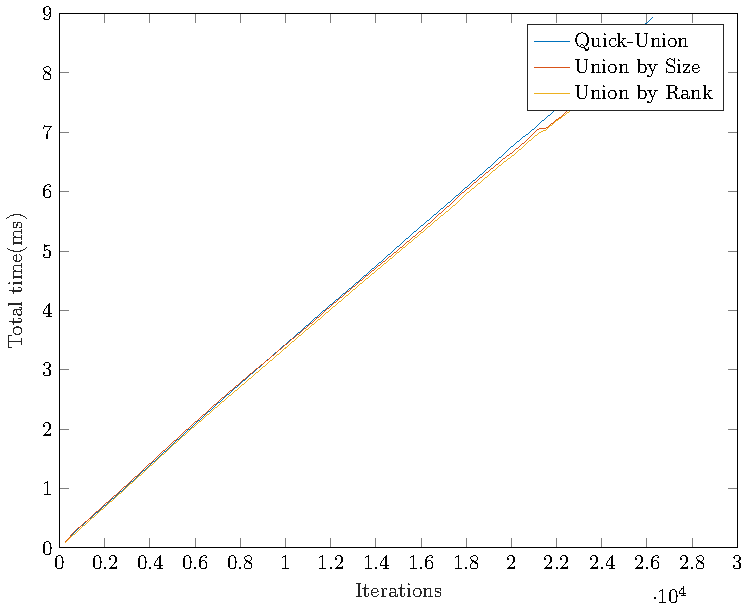
\includegraphics[width=\textwidth]{../images/plotPSFull5000_time(ms).pdf}
        \caption{Total Time with different union strategies with $n = 5000$ using Path Splitting}
    \end{subfigure}%
    \hfill
    % Subfigure 3
    \begin{subfigure}{0.32\textwidth}
        \centering
        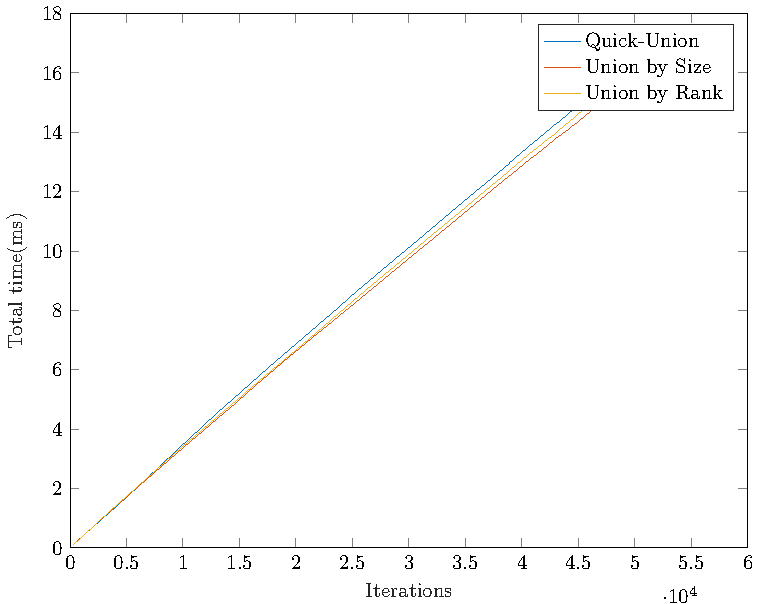
\includegraphics[width=\textwidth]{../images/plotPSFull10000_time(ms).pdf}
        \caption{Total Time with different union strategies with $n = 10000$ using Path Splitting}
    \end{subfigure}

    \begin{subfigure}{0.32\textwidth}
        \centering
        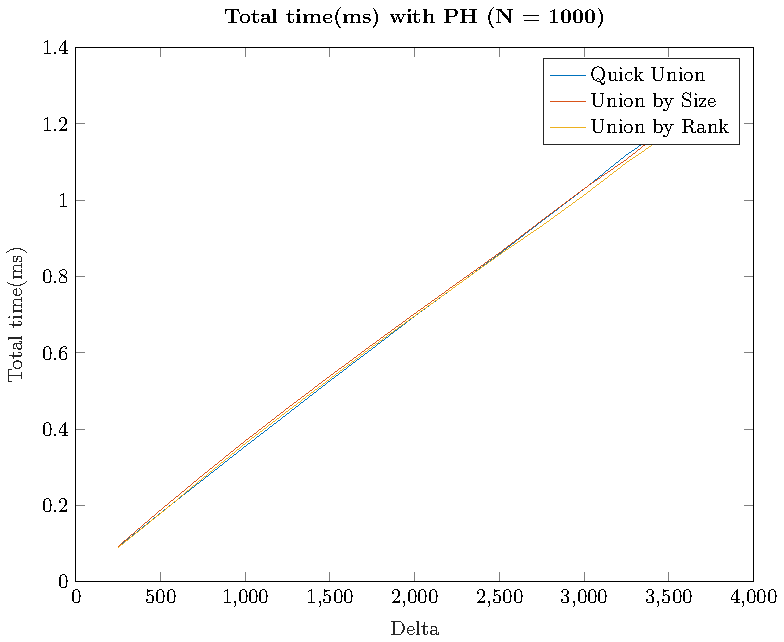
\includegraphics[width=\textwidth]{../images/plotPHFull1000_time(ms).pdf}
        \caption{Total Time with different union strategies with $n = 1000$ using Path Halving}
    \end{subfigure}%
    \hfill
    % Subfigure 2
    \begin{subfigure}{0.32\textwidth}
        \centering
        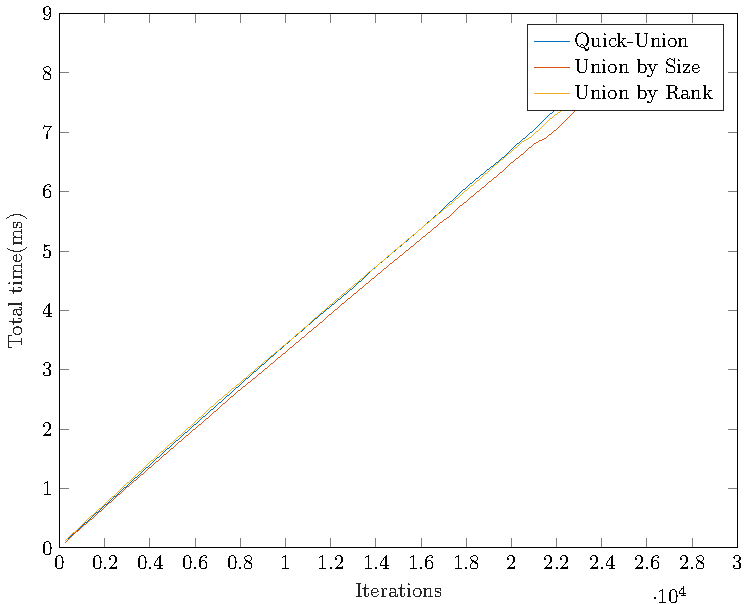
\includegraphics[width=\textwidth]{../images/plotPHFull5000_time(ms).pdf}
        \caption{Total Time with different union strategies with $n = 5000$ using Path Halving}
    \end{subfigure}%
    \hfill
    % Subfigure 3
    \begin{subfigure}{0.32\textwidth}
        \centering
        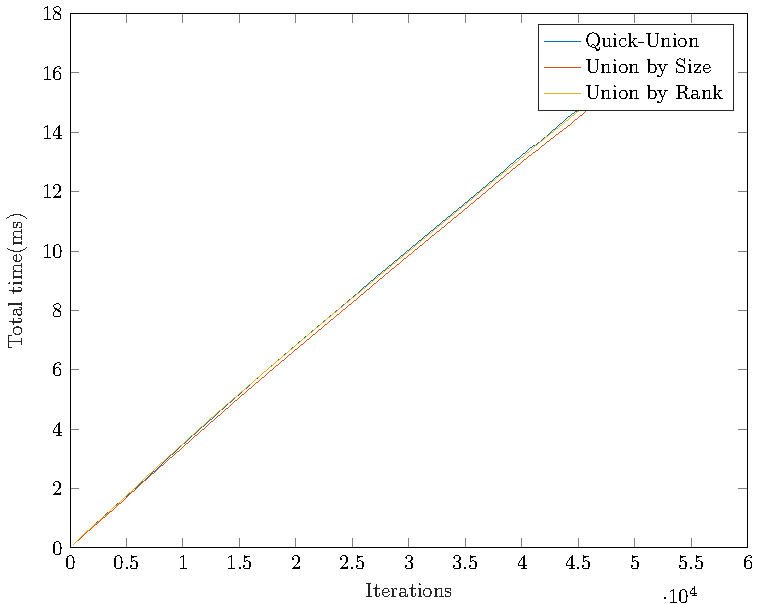
\includegraphics[width=\textwidth]{../images/plotPHFull10000_time(ms).pdf}
        \caption{Total Time with different union strategies with $n = 10000$ using Path Halving}
    \end{subfigure}
    \begin{subfigure}{0.32\textwidth}
        \centering
        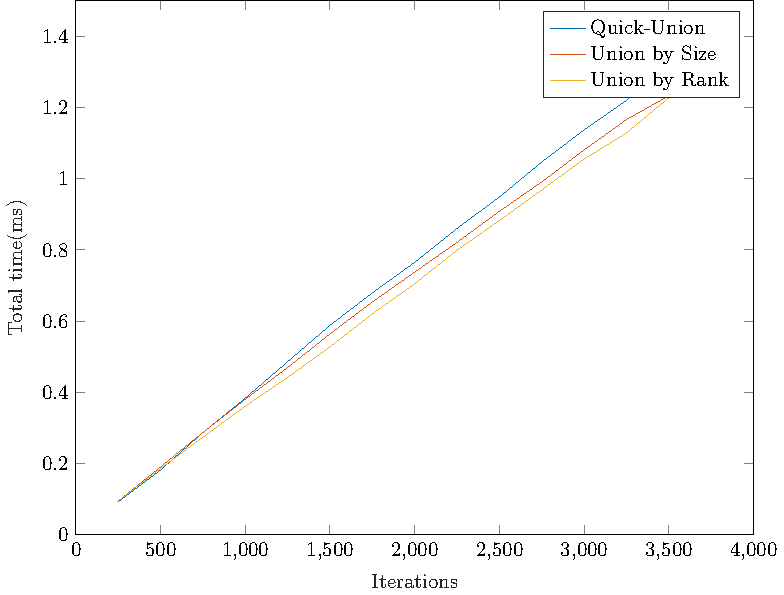
\includegraphics[width=\textwidth]{../images/plotTORFull1000_time(ms).pdf}
        \caption{Total Time with different union strategies with $n = 1000$ using Type One Reversal}
    \end{subfigure}%
    \hfill
    % Subfigure 2
    \begin{subfigure}{0.32\textwidth}
        \centering
        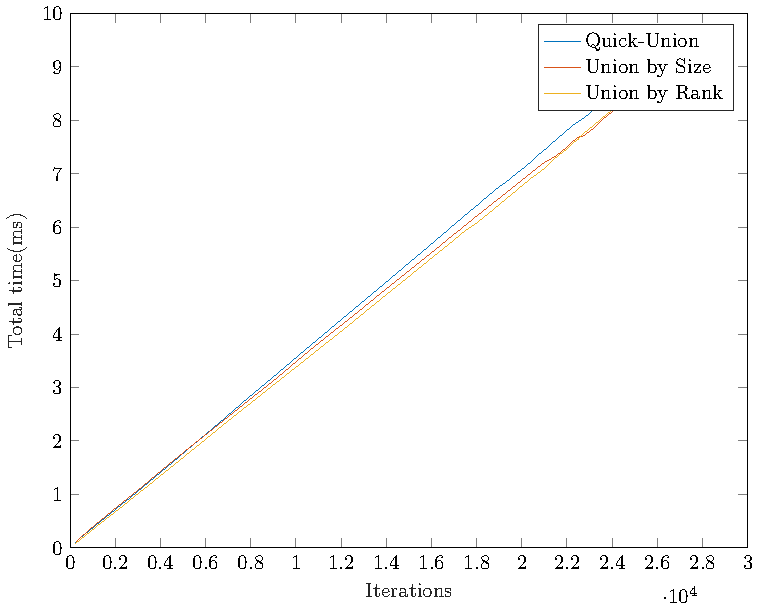
\includegraphics[width=\textwidth]{../images/plotTORFull5000_time(ms).pdf}
        \caption{Total Time with different union strategies with $n = 5000$ using Type One Reversal}
    \end{subfigure}%
    \hfill
    % Subfigure 3
    \begin{subfigure}{0.32\textwidth}
        \centering
        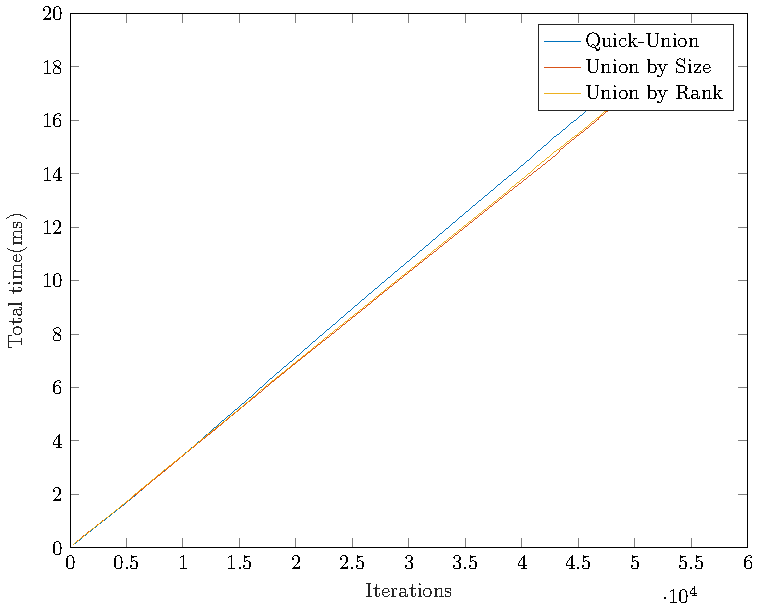
\includegraphics[width=\textwidth]{../images/plotTORFull10000_time(ms).pdf}
        \caption{Total Time with different union strategies with $n = 10000$ using Type One Reversal}
    \end{subfigure}

    \caption{Total time using different heuristics}
    \label{fig:timeH}
\end{figure}


From a theoretical analysis\cite{tarjan1984worst}, we know that Union-Find can have an amortized cost (using heuristics on both compression (full compression/splitting/halving) and unions) of \( O(m \hspace{2px} \alpha(n,m)) \), where \( \alpha \) is the inverse Ackermann function, $m$ is the number of operations we want to perform and $n$ the number of disjoint blocks. Without compression (or using type one reversal), we can achieve \( O(m \log n) \). We may need a larger input size in order to see a noticeable difference, only with those sizes we cannot see any time difference, although we really saw it calculating metrics.

